\begin{flalign*}
& A\ddot{\v q} + C \v q = \v Q = \ddot \xi_i + \omega^2 \xi_i = \tilde Q_i, \quad i = 1, \ldots, n &\\
& 1)\; \v Q = \v F\cos \omega t, \quad Q_i = \mu_i \cos \omega t \qquad \tilde Q = U^T\v F &\\
& \ddot \xi_i + \omega_i^2 \xi_i = \mu_i\cos \omega t &\\
& \left[ 
\begin{array}{ll}
\omega \neq \omega_i,\; \forall i = 1, \ldots, n & \xi_i = \alpha_i \cos (\omega_it + \beta_i) + \frac{\mu_i}{\omega_i^2 - \omega^2} \cos \omega t \\
\omega = \omega_k,\; \mu_k = 0, & \xi_k = \alpha_k \cos(\omega_kt + \beta_k) + \frac{\mu_k}{2\omega} \sin \omega t
\end{array}
\right. &\\
& 2)\; \v Q \text{ периодично по $t$: } (\v Q(t + T) = \v Q(t), \forall t \in (0; +\infty)) &\\
& \v Q(t) = \v F\left(a_0 + \sum_{k = 1}^{+\infty} A_k \cos\left(\frac{2\pi k t}{T} + Q_k \right)\right) &\\
& \v q = \v q_{\text{одн}} + \sum_{k = 0}^{+\infty}\v q_\text{ч}^{(k)} &\\
& \omega_i = \frac{2\pi k}{T}
\end{flalign*}

\begin{xmp}
\begin{flalign*}
& \ddot x + k \dot x + \omega_0^2 x = f \sin \omega t, \; k > 0 &\\
& x = 0 \text{ --- равновесие (установившееся асимптотически) свободной системы} &\\
& \lim_{x \rightarrow +\infty} x_\text{одн} = 0 &\\
& x_\text{ч} = R\sin(\omega t + \varphi) &\\
& \dot x_\text{ч} = R\omega\cos(\omega t + \varphi) &\\
& \ddot x_\text{ч} = - R\omega^2\sin(\omega t + \varphi) &\\
& R(\omega_0^2 - \omega^2)\sin(\omega t + \varphi) + KR\omega\cos(\omega t + \varphi) = f\sin \omega t &\\
& R = \frac{f}{\sqrt{(\omega^2 - \omega^2)^2 + k^2 \omega^2}}, \quad \varphi = - \arctg \frac{k\omega}{\omega_0^2 - \omega^2} &\\
& ((\omega_0^2 - \omega^2) + k^2\omega^2)'_\omega = -2(\omega_0^2 - \omega^2)\cdot 2\omega + 2k^2\omega = 0 \Leftrightarrow 
\left[\begin{array}{l}
\omega = 0 \\ 
\omega^2 = \omega_0^2 - \frac{k^2}{2} \\
\end{array}\right. &\\
\end{flalign*}
\begin{figure}[H]
	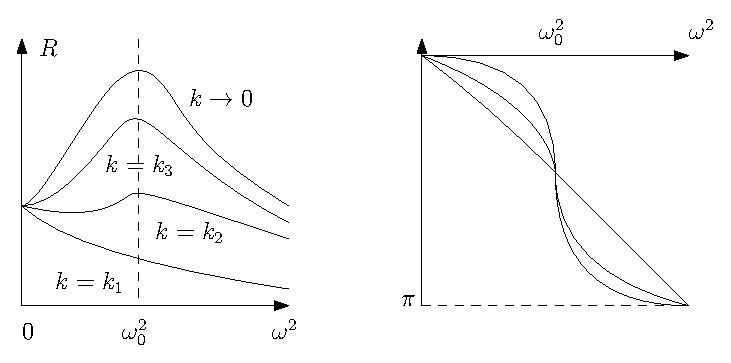
\includegraphics{6_1.eps}
\end{figure}
\end{xmp}

\begin{flalign*}
& \frac{d}{dt}\pd{l}{\dot q} - \pd{L}{\v q} = \v Q^* + \v Q(t) &\\
& \v Q^* = B \dv q,\; B = const &\\
& \v q = 0 \text{ --- устойчиво асимптотически} &\\
& \det(A\lambda^2 + B\lambda + C) = 0 \Leftrightarrow \re \lambda_i < 0, \; i = 1, \ldots, n &\\
& P(\lambda) = A\lambda^2 + B\lambda + C &\\
& \v Q(t) = \v F \sin \omega t \Rightarrow \v Q(t) = \v Fe^{i\omega t} &\\
& \v q = \v q_\text{ч} = \v h e^{i\omega t} \quad \dv q = \v h i \omega e^{i \omega t} \quad \ddot{\v q} = \v h(i\omega)^2 e^{i\omega t} &\\
& D(i\omega) \v h = \v F \quad \det D(i\omega) \neq 0 &\\
& \v h = [D(i\omega)]^{-1} \v F = W(i\omega) \v F, \; W(i\omega) = (w_{kj}), \; k,j = 1, \ldots, n &\\
& w_{kj} = |w_{kj}|e^{i\arg \omega_{kj}} = R_{kj}e^{i\varphi_{kj}} &\\
& R_{kj} = |w_{kj}| \qquad \v q = W(i\omega)\v F e^{i\omega t} &\\
& \varphi_{kj} = \arg \omega_{kj} \qquad \sum_{j = 1}^n w_{kj}F_j e^{i\omega t} = \sum R_{kj} F_j e^{i(\omega t + \varphi_{kj})}
\end{flalign*}

\section{Гамильтонова механика}
\subsection{Преобразования Лежандра}
Рассмотрим $X(\v x): \; \R^n \rightarrow \R, \; X(\v x) \in C$.
\begin{flalign*}
& \det \pd{^2 X}{x^2} \neq 0 &\\
& \v y = \v f(\v x) = \pd{X}{x} &\\
& \Rightarrow \v x = \v f^{-1}(\v y) = \v x(\v y) &\\
& Y(\v y) = ((\v x, \v y) - X(\v x)) \vert_{\v x = \v x(\v y)} &\\
\end{flalign*}

\begin{df}
$Y(\v y)$ --- преобразование Лежандра функции $X(\v x)$ по переменной $\v x$.
\end{df}
Свойства преобразований Лежандра\footnote{Возможно, тут чего-то не хватает}:
\begin{enumerate}
\item Инвалютивность.
\begin{flalign*}
& X,\v x \rightarrow Y, \; \v y \rightarrow X, \v x &\\
& \pd{Y}{y_i} = x_i + \left( \pd{\v x}{y_i}, \v y \right) - \left( \pd{X}{\v x}, \pd{\v x}{y_i} \right) = &\\
& x_i + \left(\underbrace{\v y - \pd{X}{\v x}}_0, \pd{\v x}{y}\right) = x_i, \; i = 1, \ldots, n \Rightarrow &\\
& \Rightarrow \v x = \pd{Y}{\v y}
\end{flalign*}
\item \begin{flalign*}
& \pd{^2 Y}{\v y^2} = \pd{\v x}{\v y} = \left( \pd{\v y}{\v x} \right)^{-1} = \left( \pd{^2 X}{\v x^2} \right)^{-1} &\\
& \det \pd{^2 Y}{\v y^2} = \left( \det \pd{^2 X}{\v x^2} \neq 0 \right) &\\
\end{flalign*}
\item \begin{flalign*}
& \v x, X \rightarrow \v y, Y = [(\v x, \v y) - X(\v x)]\vert_{\v x = f'(\v y)} \rightarrow \v z, Z &\\
& \v y = \v f_2(\v z),\; \v z = \v x,\; \v y = f_2^{-1}(\v x),\; f'(f_2^{-1}) = \v x &\\
& Y(\v y)_{\v y = f_2^{-1}(\v x)} = (\v x, \v y \vert_{\v y = f_2^{-1}(\v x)}) - X(\v x) &\\
& X(\v x) = [(\v x, \v y) - Y(\v y)]\vert_{\v y = \v y(x)}
\end{flalign*}
\item \begin{flalign*}
& X = X(\v x, \alpha), \alpha \in \R &\\
& Y = Y(\v y, \alpha) &\\
& \pd{X}{\alpha} = -\pd{Y}{\alpha} &\\
& Y(\v y, \alpha) = ((\v x, \v y(\v x, \alpha)) - X(\v x, \alpha)) \vert_{\v x = \v x(\v y, \alpha)} &\\
& \pd{Y}{\alpha} = \left( \pd{\v x}{\alpha}, \v y \right) - \left( \pd{X}{\v x}, \pd{\v x}{\alpha} \right) - \pd{X}{\alpha} =  &\\
& = \left( \pd{\v x}{\alpha}, \underbrace{\v y - \pd{X}{\v x}}_0 \right) - \pd{X}{\alpha} = - \pd{X}{\alpha}
\end{flalign*}
\end{enumerate}

Повторим это с лагранжианом.
\begin{flalign*}
& L = L(q, \dot q, t)
\end{flalign*}
\begin{df}
$p = \pd{L}{\dot q}$ --- обобщенный импульс.
\end{df}
\begin{flalign*}
& \det \pd{^2 L}{\dot q^2} \neq 0 \Rightarrow \dot q = \dot q(q, p, t) &\\
& H(q, p, t) = [(\dot q, p) - L(q, \dot q, t)]\vert_{\dot q = \dot q(q, p, t)} &\\
\end{flalign*}

\begin{df}
$H$ --- гамильтониан (функция Гамильтона).
\end{df}
\begin{df}
$(q, p, t)$ --- канонические переменные (параметры Гамильтона).
\end{df}
\begin{teo}
В канонических переменных уравнения движения имеют вид
\[
	\begin{cases}
	\dot q = \pd{H}{p} \\
	\dot p = -\pd{H}{q} \\
	\end{cases}
\]
\end{teo}
\begin{proof}
\begin{flalign*}
& \text{Инвалютивность} \Rightarrow \dot q = \pd{H}{p} &\\
& \dot p = \frac{dp}{dt} = \frac{d}{dt}\pd{L}{\dot q} = \frac{L}{q} = -\pd{H}{q}
\end{flalign*}
\end{proof}

\begin{df}
\begin{flalign*}
& \dv x = \v F(\v x, t) \v x \in \R^{2n} \text{ --- гамильтонова система, если} &\\
& \v x = (q_1, \ldots, q_n, p_1, \ldots, p_n)^T \quad \exists H = H(q, p): &\\
& \v F = \left( \pd{H}{p_1}, \ldots, \pd{H}{p_n}, -\pd{H}{q_1}, \ldots, -\pd{H}{q_n} \right)^T
\end{flalign*}
\end{df}
ПРИМЕР